%!TEX root = main.tex
\setcounter{chapter}{4}
\setcounter{section}{5}
\setcounter{theorem}{0}
\setcounter{equation}{0}

\lectureheader{161}{Calculus I}{Applied optimization}{\textit{Thomas' Calculus} \thesection}

\begin{remark}
To solve an applied optimization problem, do the following (iteratively).
\begin{enumerate}
\item Read the problem carefully.
\item Introduce/define notation with appropriate units.
\item Sketch a well-labeled diagram of the situation.
\item Identify the quantity to be optimized (maximized or minimized).
\item Use your diagram to develop a model.
\begin{enumerate}
\item Express the quantity to be optimized as the output of some \textbf{objective function}.
\item Note any constraints the problem imposes on the domain of the objective function.
\end{enumerate}
\item Use the techniques of calculus to determine the global maximum or global minimum of the objective function over its domain.
Note: You may be more interested in the ``location" of the global extreme than the extreme value itself.
\end{enumerate}
\end{remark}

\begin{example}
An open-top box is to be made by cutting small congruent squares from the corners of a 12-\si{in.} by 12-\si{in.} sheet of tin and bending up the sides.
How large should the squares be to make the box hold as much as possible?
\end{example}

\newpage

\begin{example}
You have been asked to design a 1-liter can shaped like a right circular cylinder.
What dimensions will use the least material?
\end{example}

\newpage

%\begin{remark}[Fermat's principle in optics]
%The speed of light depends on the medium through which it travels.
%Light travels from one point to another along a path for which the time of travel is minimum.
%\end{remark}

\begin{example}[Snell's law of refraction]
Suppose that light passes through one medium where its speed is $c_1$ into another where its speed is $c_2$.
According to Fermat's principle in optics, light will travel from a point $A$ in the first medium to a point $B$ in the second medium by a path $APB$ that minimizes the total travel time.  
See the diagram below.
Show that
\begin{equation*}
\frac{\sin\theta_1}{c_1} = \frac{\sin\theta_2}{c_2}
\end{equation*}
where $\theta_1$ is the angle of incidence and $\theta_2$ is the angle of refraction.
\begin{flushright}
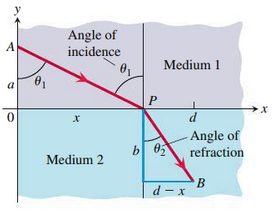
\includegraphics[width=3in]{img/snell_diagram}
\end{flushright}
\end{example}
